\documentclass[dvipsnames]{beamer}\usepackage[]{graphicx}\usepackage[]{color}
%% maxwidth is the original width if it is less than linewidth
%% otherwise use linewidth (to make sure the graphics do not exceed the margin)
\makeatletter
\def\maxwidth{ %
  \ifdim\Gin@nat@width>\linewidth
    \linewidth
  \else
    \Gin@nat@width
  \fi
}
\makeatother

\definecolor{fgcolor}{rgb}{0.345, 0.345, 0.345}
\newcommand{\hlnum}[1]{\textcolor[rgb]{0.686,0.059,0.569}{#1}}%
\newcommand{\hlstr}[1]{\textcolor[rgb]{0.192,0.494,0.8}{#1}}%
\newcommand{\hlcom}[1]{\textcolor[rgb]{0.678,0.584,0.686}{\textit{#1}}}%
\newcommand{\hlopt}[1]{\textcolor[rgb]{0,0,0}{#1}}%
\newcommand{\hlstd}[1]{\textcolor[rgb]{0.345,0.345,0.345}{#1}}%
\newcommand{\hlkwa}[1]{\textcolor[rgb]{0.161,0.373,0.58}{\textbf{#1}}}%
\newcommand{\hlkwb}[1]{\textcolor[rgb]{0.69,0.353,0.396}{#1}}%
\newcommand{\hlkwc}[1]{\textcolor[rgb]{0.333,0.667,0.333}{#1}}%
\newcommand{\hlkwd}[1]{\textcolor[rgb]{0.737,0.353,0.396}{\textbf{#1}}}%

\usepackage{framed}
\makeatletter
\newenvironment{kframe}{%
 \def\at@end@of@kframe{}%
 \ifinner\ifhmode%
  \def\at@end@of@kframe{\end{minipage}}%
  \begin{minipage}{\columnwidth}%
 \fi\fi%
 \def\FrameCommand##1{\hskip\@totalleftmargin \hskip-\fboxsep
 \colorbox{shadecolor}{##1}\hskip-\fboxsep
     % There is no \\@totalrightmargin, so:
     \hskip-\linewidth \hskip-\@totalleftmargin \hskip\columnwidth}%
 \MakeFramed {\advance\hsize-\width
   \@totalleftmargin\z@ \linewidth\hsize
   \@setminipage}}%
 {\par\unskip\endMakeFramed%
 \at@end@of@kframe}
\makeatother

\definecolor{shadecolor}{rgb}{.97, .97, .97}
\definecolor{messagecolor}{rgb}{0, 0, 0}
\definecolor{warningcolor}{rgb}{1, 0, 1}
\definecolor{errorcolor}{rgb}{1, 0, 0}
\newenvironment{knitrout}{}{} % an empty environment to be redefined in TeX

\usepackage{alltt}
\usepackage{color} % for colors
\usepackage{graphicx}
\usepackage{hyperref}

\hypersetup{
    bookmarks=true,         % show bookmarks bar?
    unicode=false,          % non-Latin characters in Acrobat?s bookmarks
    pdftoolbar=true,        % show Acrobat?s toolbar?
    pdfmenubar=true,        % show Acrobat?s menu?
    pdffitwindow=false,     % window fit to page when opened
    pdfstartview={FitH},    % fits the width of the page to the window
    pdftitle={My title},    % title
    pdfauthor={Author},     % author
    pdfsubject={Subject},   % subject of the document
    pdfcreator={Creator},   % creator of the document
    pdfproducer={Producer}, % producer of the document
    pdfkeywords={keyword1} {key2} {key3}, % list of keywords
    pdfnewwindow=true,      % links in new PDF window
    colorlinks=true,       % false: boxed links; true: colored links
    linkcolor=red,          % color of internal links (change box color with linkbordercolor)
    citecolor=green,        % color of links to bibliography
    filecolor=magenta,      % color of file links
    urlcolor=blue         % color of external links
}
% \usepackage{beamerthemesplit} // Activate for custom appearance

\usecolortheme{beaver}
\title{E-411-PRMA}
\subtitle{Lecture 1}
\author{Christopher David Desjardins}
\date{17 August 2015}
\IfFileExists{upquote.sty}{\usepackage{upquote}}{}
\begin{document}







\frame{\titlepage}

%\section[Outline]{}
%\frame{\tableofcontents}

\begin{frame}
\centerline{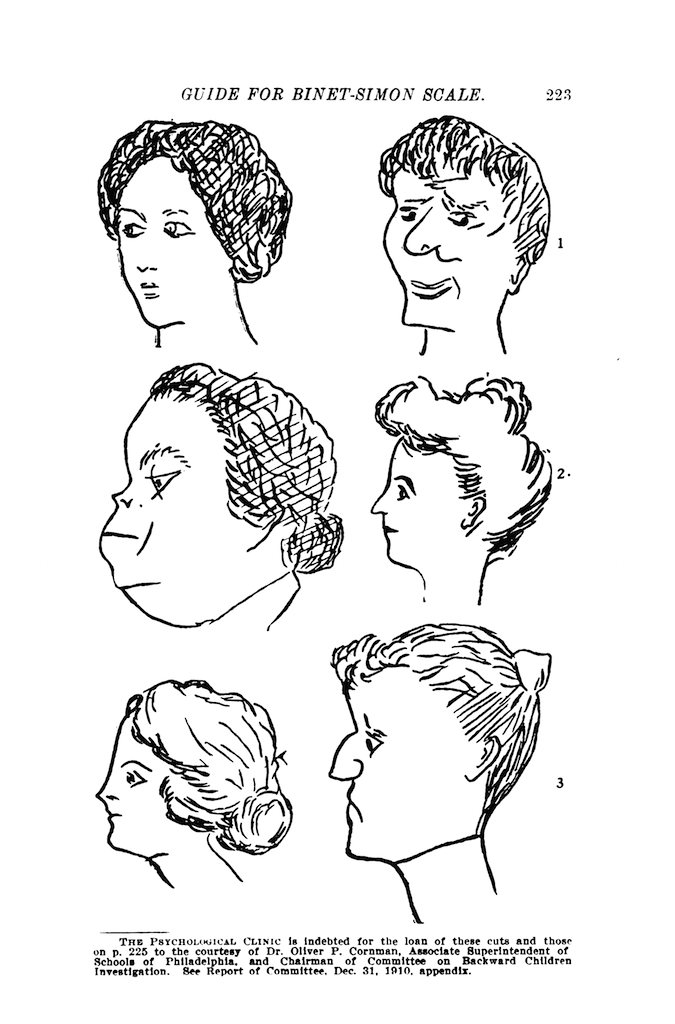
\includegraphics[scale=.35]{images/binet2.png}}
\end{frame}

\begin{frame}
\centerline{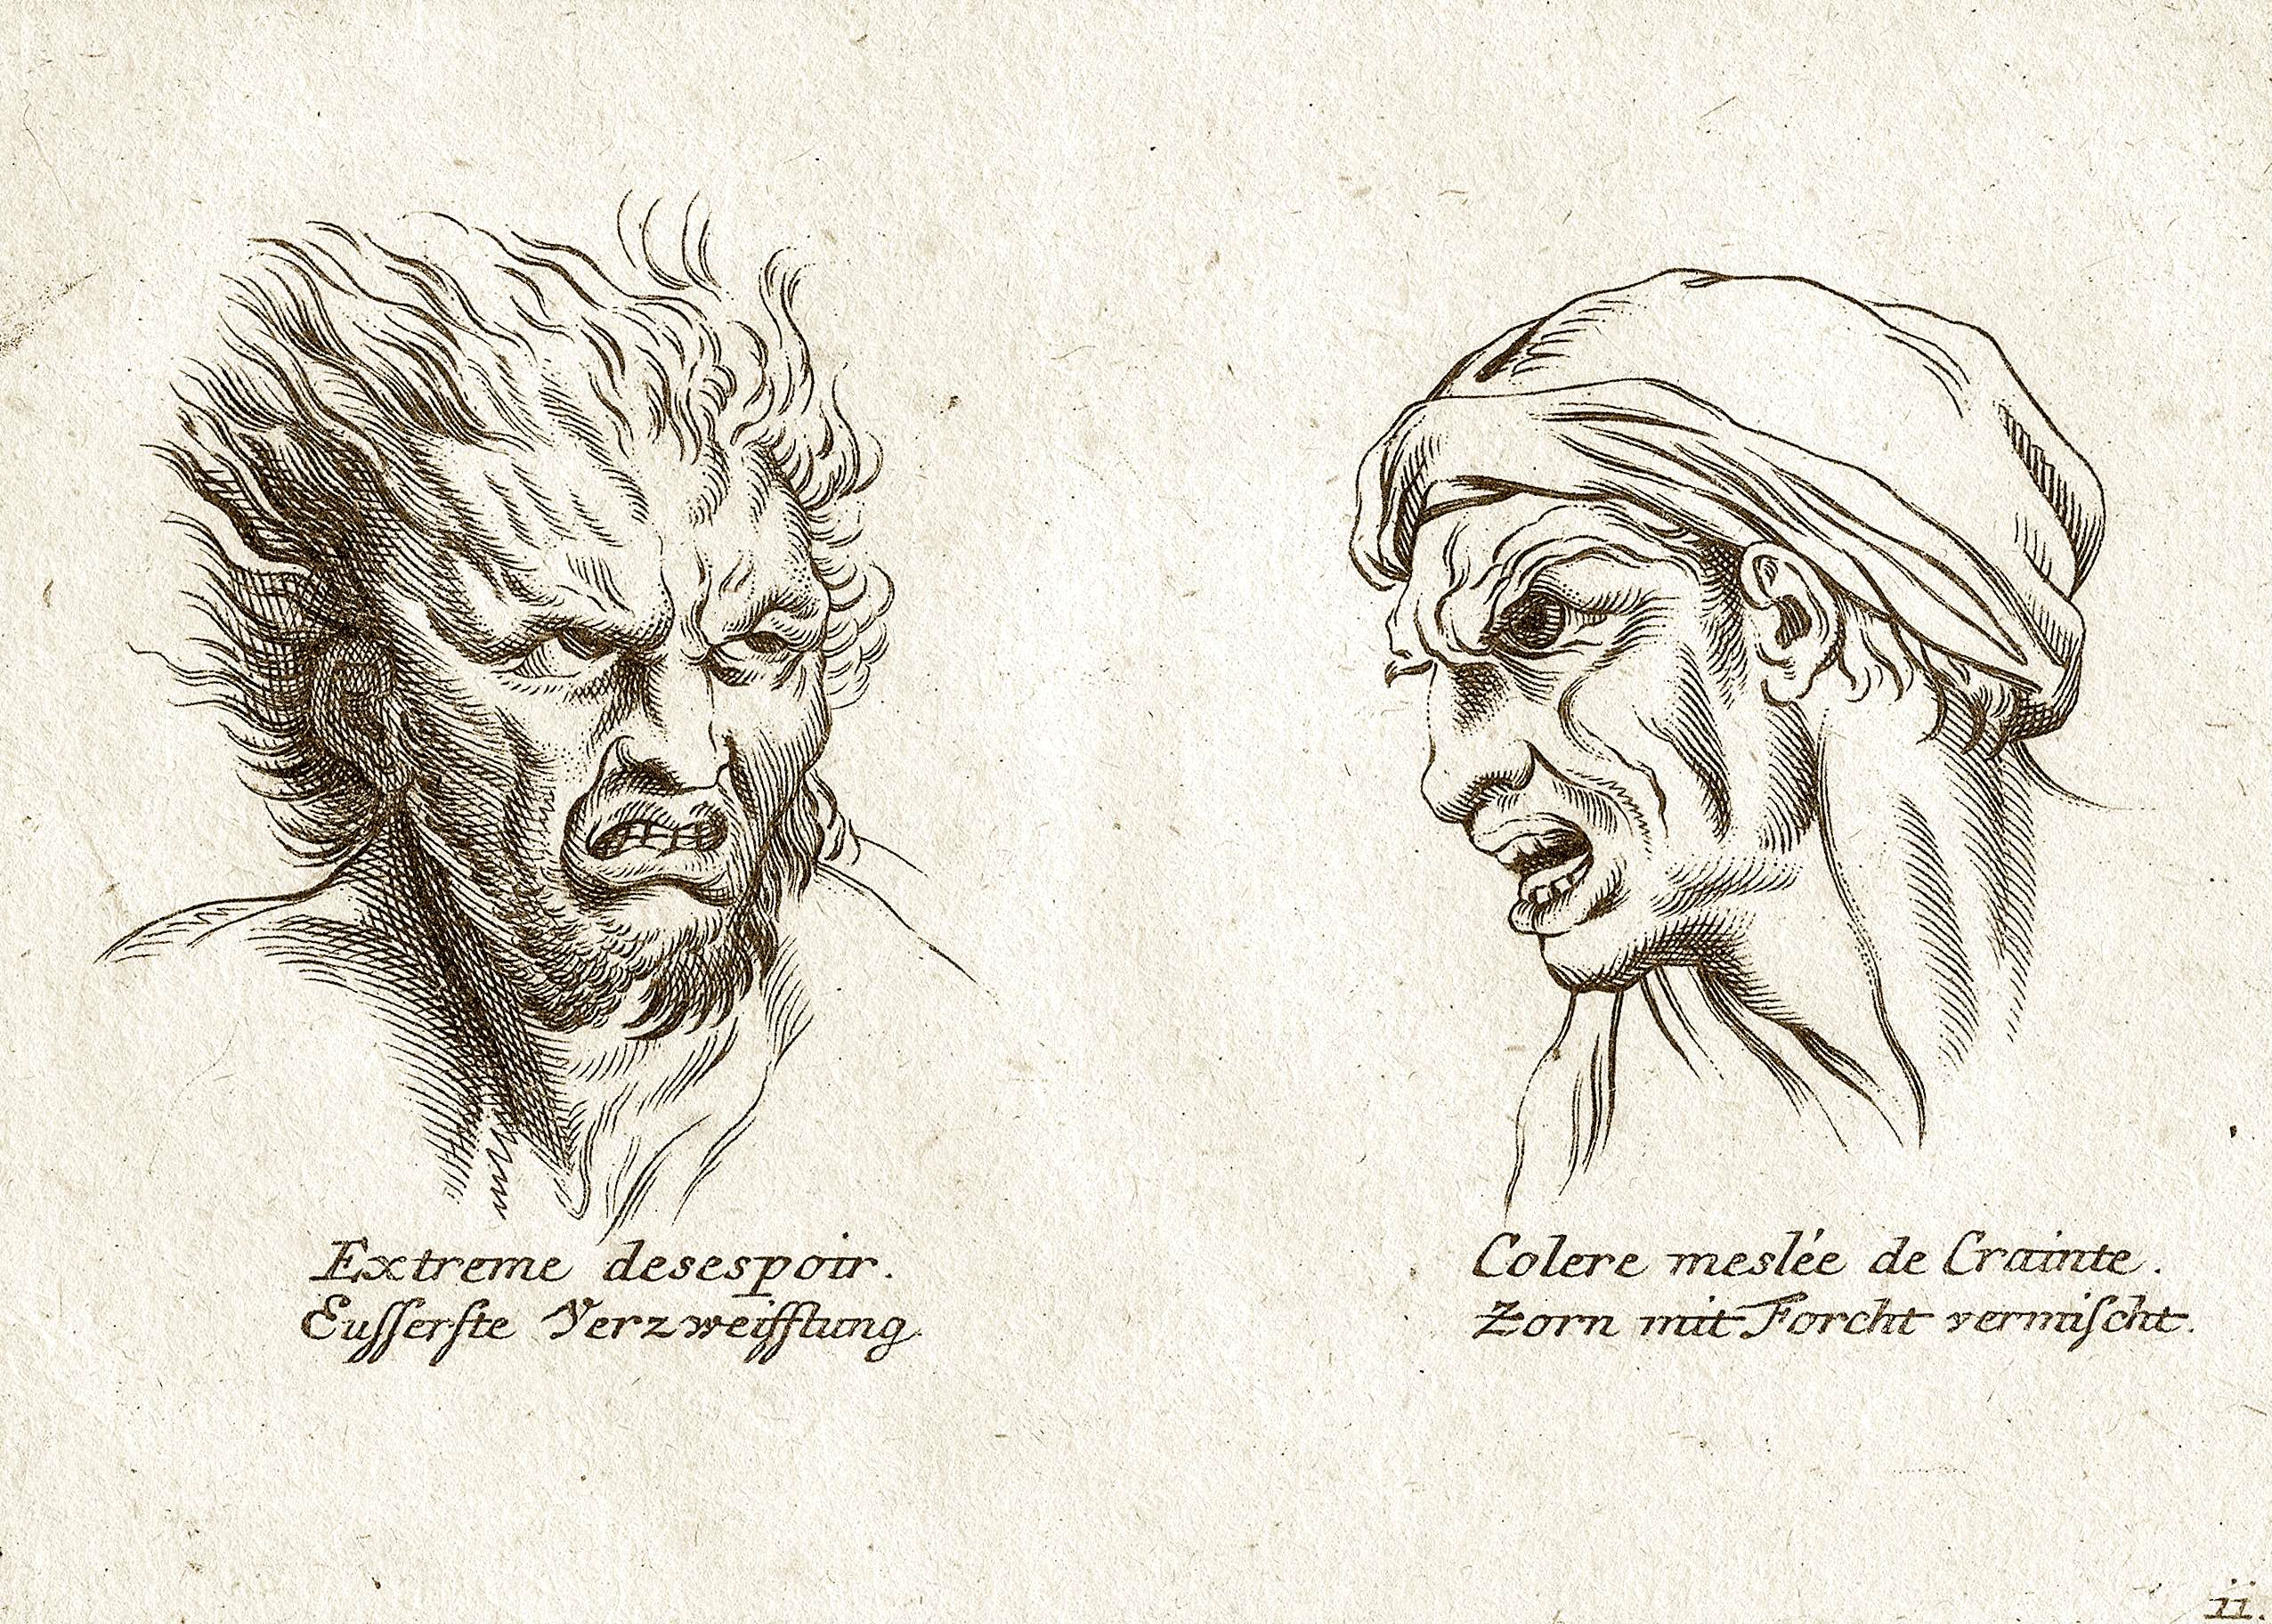
\includegraphics[scale=.15]{images/physiognomy.jpg}}
\end{frame}

\begin{frame}
\centerline{
\includegraphics[scale=.2]{images/sat.png}}
\end{frame}

\frame
{
  \frametitle{E-411-PRMA}

\begin{itemize}
  	\item \textbf{Topics}
		\begin{itemize}
			\item Statistics, Classical Test Theory, Reliability, Validity, Item Response Theory, Generalizability Theory, Equating, and assessments/issues specific to various fields
			\end{itemize}
			\item \textbf{Assessments}
			\begin{itemize}
			  \item R computer assignments (30\%)
			  \item Item writing activity (5\%)
			  \item Midterm exam (25\%)
			  \item \textcolor{red}{Final exam (50\%)}
		\end{itemize}  
  \end{itemize}
}

\begin{frame}
    \begin{center}
    	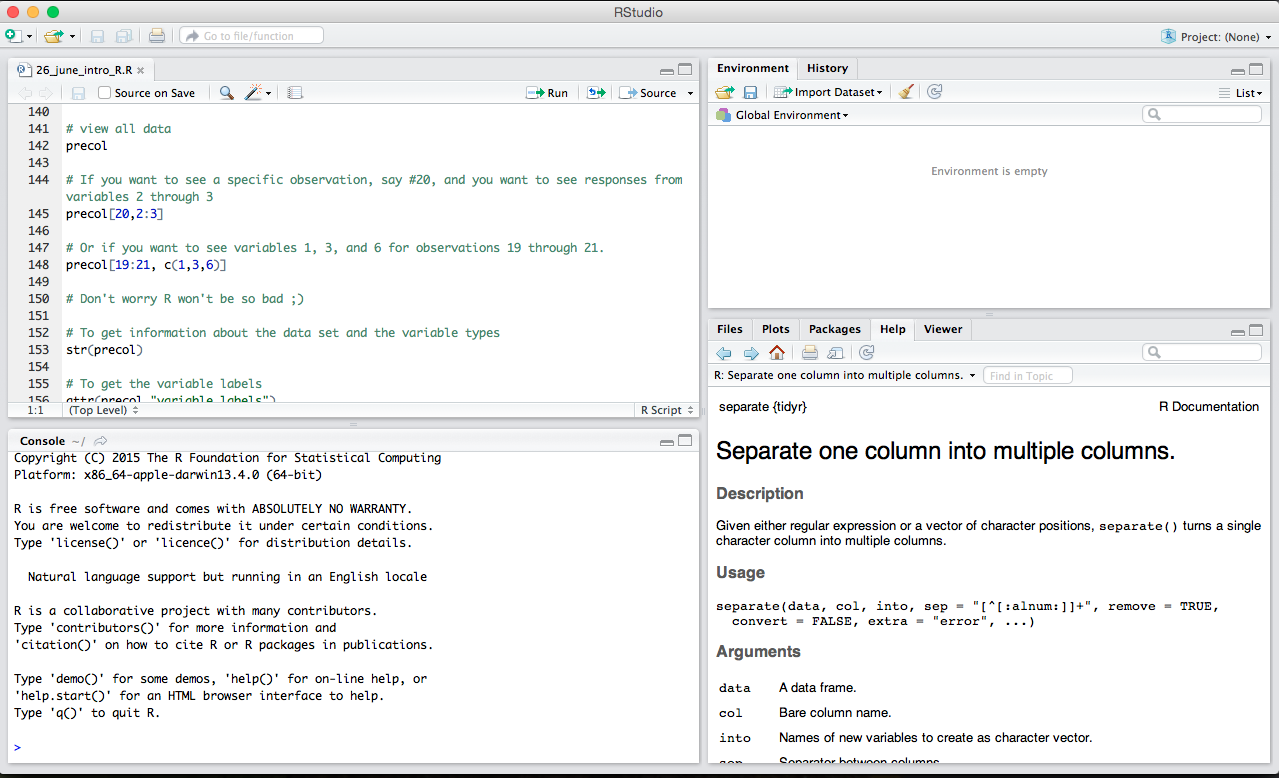
\includegraphics[width=\textwidth]{images/rstudio.png}
    \end{center}
\begin{flushright}
\href{https://www.r-project.org}{R: \underline{https://www.r-project.org}}

\href{https://www.rstudio.com}{RStudio: \underline{https://www.rstudio.com}}
\end{flushright}
\end{frame}


\frame{
\frametitle{Why should I learn R?}
\begin{itemize}
	\item<1->It's free and open-source 
	\item<2->Statistics and psychometrics analyses
 	\item<3->Helps you learn statistics better
	\item<4-> Learn reproducible research
	\item<5-> Extremely marketable skill
 	\item<6->High quality graphics
	\item<7-> Everyone is doing it
 	\item<8->Steep learning curve
	\begin{itemize}
 		\item<9->\color{RoyalBlue}{Will provide nearly all the code}
	\end{itemize}
 	\item<10->\color{red}{No SPSS in this class}
\end{itemize}
}

\frame{
\frametitle{Resources for R}
\begin{itemize}
	\item Icelandic resources
		\begin{itemize}
			\item[] \url{http://kennslubanki.hi.is/search/efni/r}
			\item[] \url{http://kennslubanki.hi.is/tolfraedi/myndbond/rrstudio-inngangur}
			\item[] \url{http://kennslubanki.hi.is/tolfraedi/myndbond/rrstudio-fyrstu-skrefin}
		\end{itemize}
	\item Please watch the last two videos before next class
	\item Please install R and RStudio before next class
	\item Next class will be an R workshop
\end{itemize}
}

\frame{
\frametitle{Concepts}
\begin{itemize}
	\item[]<1-> What is \textbf{measurement}?
	\begin{itemize}
		\item[]<4-> Assignment of numerical values based on a set of rules
	\end{itemize}
	\vspace{.5cm}
	\item[]<2-> What is a \textbf{test}?
		\begin{itemize}
		\item[]<5-> An instrument used to measure
		\end{itemize} 
	\vspace{.5cm}
	\item[]<3-> What is a \textbf{scale}?
			\begin{itemize}
		\item[]<6->A set of numbers used to categorize or quantify variables ("things")
			\begin{itemize}
		\item[]<7-> \textbf{Nominal}
		\item[]<7-> \textbf{Ordinal}
		\item[]<7-> \textbf{Ratio}
		\item[]<7-> \textbf{Interval}
				\end{itemize} 
				\end{itemize} 
\end{itemize}
}

\frame{
\frametitle{What kind of scales are these?}
\begin{itemize}
	\item Temperature
	\item Height
	\item Intelligence Quotient
	\item Color
	\item Ethnic group
	\item Likert-type items
	\item Job satisfaction
\end{itemize}
}

\begin{frame}
\begin{knitrout}
\definecolor{shadecolor}{rgb}{0.969, 0.969, 0.969}\color{fgcolor}

{\centering 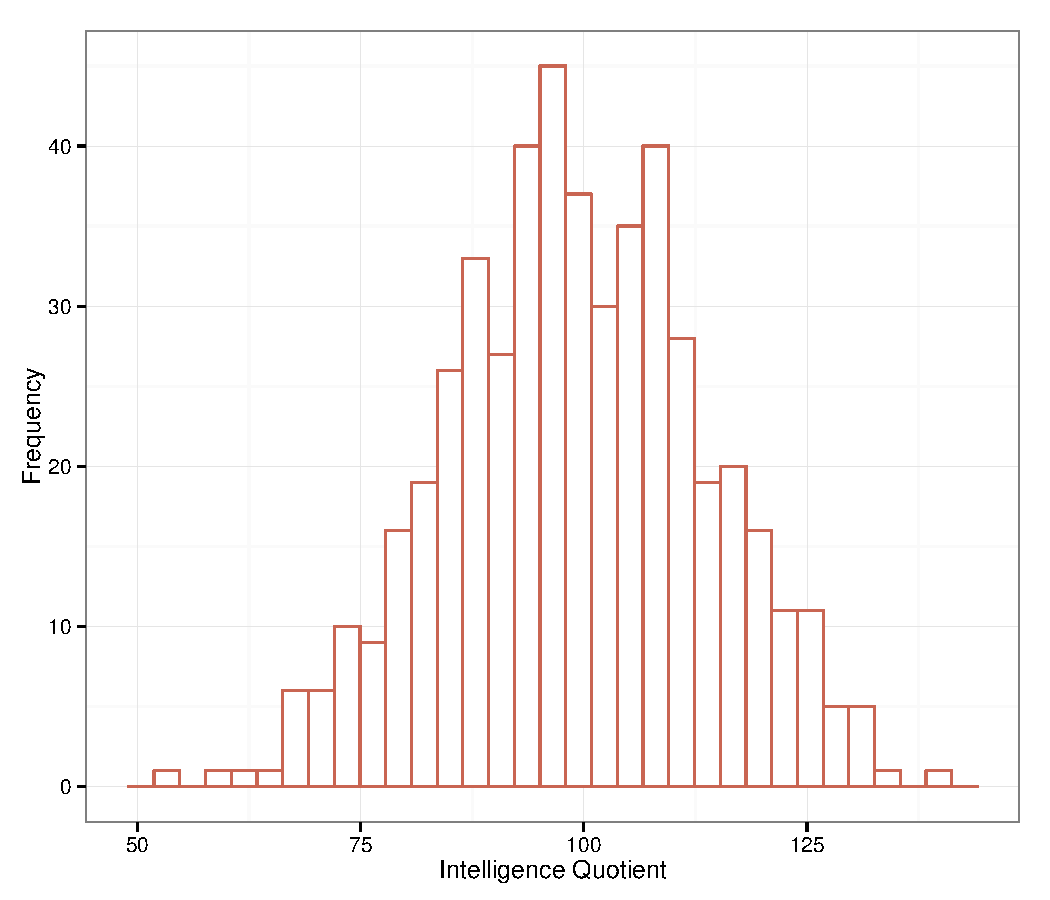
\includegraphics[width=\maxwidth]{figure/unnamed-chunk-2-1} 

}



\end{knitrout}
\end{frame}

\begin{frame}[fragile]
\begin{knitrout}
\definecolor{shadecolor}{rgb}{0.969, 0.969, 0.969}\color{fgcolor}\begin{kframe}
\begin{alltt}
\hlcom{# Load the library}
\hlkwd{set.seed}\hlstd{(}\hlnum{101}\hlstd{)}
\hlkwd{library}\hlstd{(}\hlstr{"ggplot2"}\hlstd{)}

\hlcom{# Set up the parameters}
\hlstd{sample_size} \hlkwb{<-} \hlnum{500}
\hlstd{mean} \hlkwb{<-} \hlnum{100}
\hlstd{standard_deviation} \hlkwb{<-} \hlnum{15}

\hlcom{# Generate random numbers}
\hlstd{x} \hlkwb{<-} \hlkwd{rnorm}\hlstd{(sample_size, mean, standard_deviation)}

\hlcom{# Plot the data}
\hlkwd{qplot}\hlstd{(x,} \hlkwc{fill} \hlstd{=} \hlkwd{I}\hlstd{(}\hlstr{"white"}\hlstd{),} \hlkwc{color} \hlstd{=} \hlkwd{I}\hlstd{(}\hlstr{"#c96552"}\hlstd{))} \hlopt{+}
  \hlkwd{theme_bw}\hlstd{()} \hlopt{+} \hlkwd{xlab}\hlstd{(}\hlstr{"Intelligence Quotient"}\hlstd{)} \hlopt{+}
  \hlkwd{ylab}\hlstd{(}\hlstr{"Frequency"}\hlstd{)}
\end{alltt}
\end{kframe}
\end{knitrout}
\end{frame}

\begin{frame}
\begin{knitrout}
\definecolor{shadecolor}{rgb}{0.969, 0.969, 0.969}\color{fgcolor}

{\centering 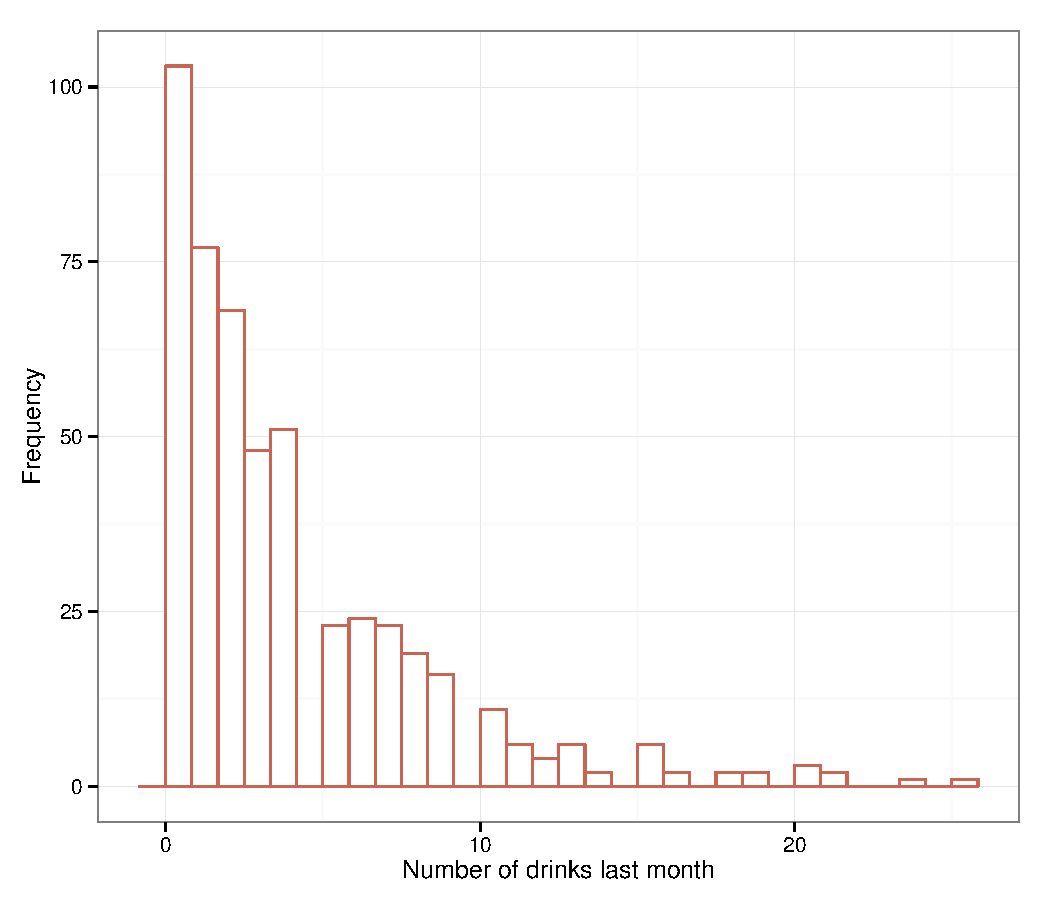
\includegraphics[width=\maxwidth]{figure/unnamed-chunk-4-1} 

}



\end{knitrout}
\end{frame}

\begin{frame}
\begin{knitrout}
\definecolor{shadecolor}{rgb}{0.969, 0.969, 0.969}\color{fgcolor}

{\centering 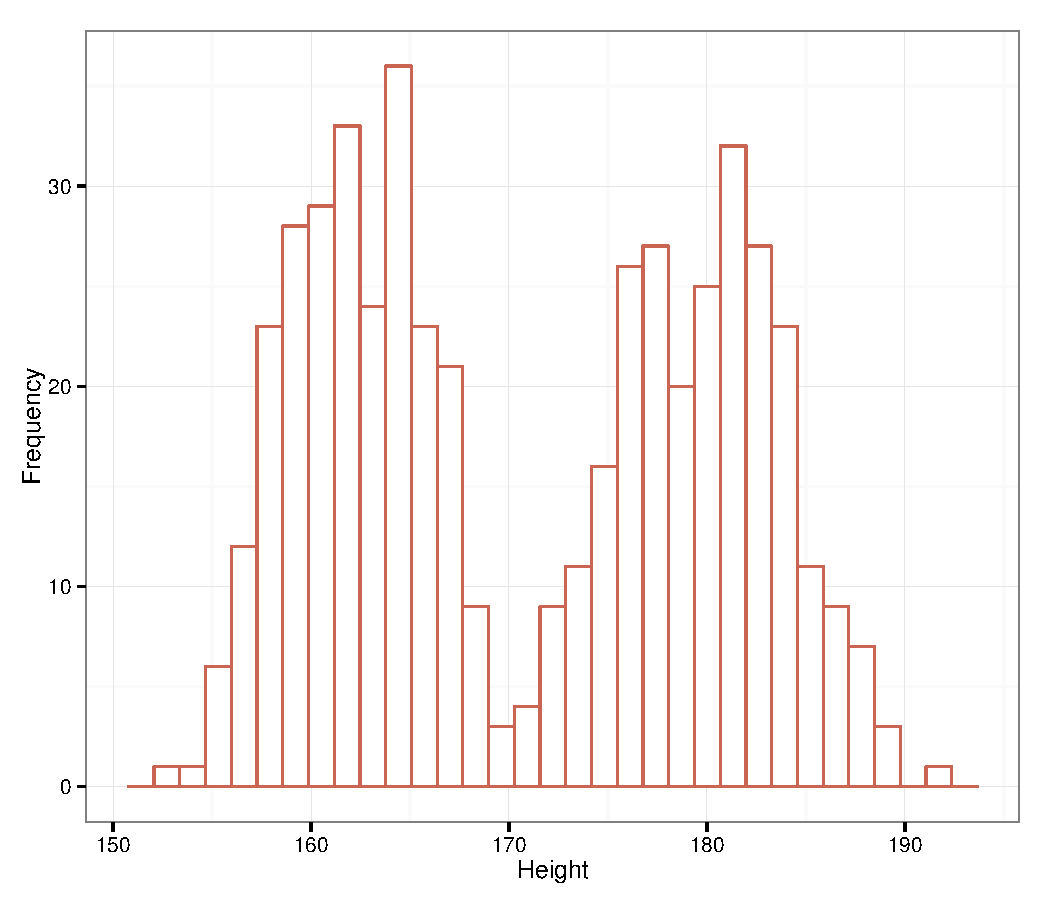
\includegraphics[width=\maxwidth]{figure/unnamed-chunk-5-1} 

}



\end{knitrout}
\end{frame}

\begin{frame}
\frametitle{Central Tendency Measures}
\begin{center}
\textbf{Mean}
$$
\bar{X} = \frac{\sum X_i}{n}
$$

\textbf{Median}
$$
\operatorname{P}(X\leq m) \geq \frac{1}{2}\text{ and }\operatorname{P}(X\geq m) \geq \frac{1}{2}
$$

\textbf{Mode}

The most frequently occurring value

\vspace{.5cm}
\textcolor{red}{Which of these statistics is most robust to outliers?}
\end{center}
\end{frame}

\begin{frame}
\begin{knitrout}
\definecolor{shadecolor}{rgb}{0.969, 0.969, 0.969}\color{fgcolor}

{\centering 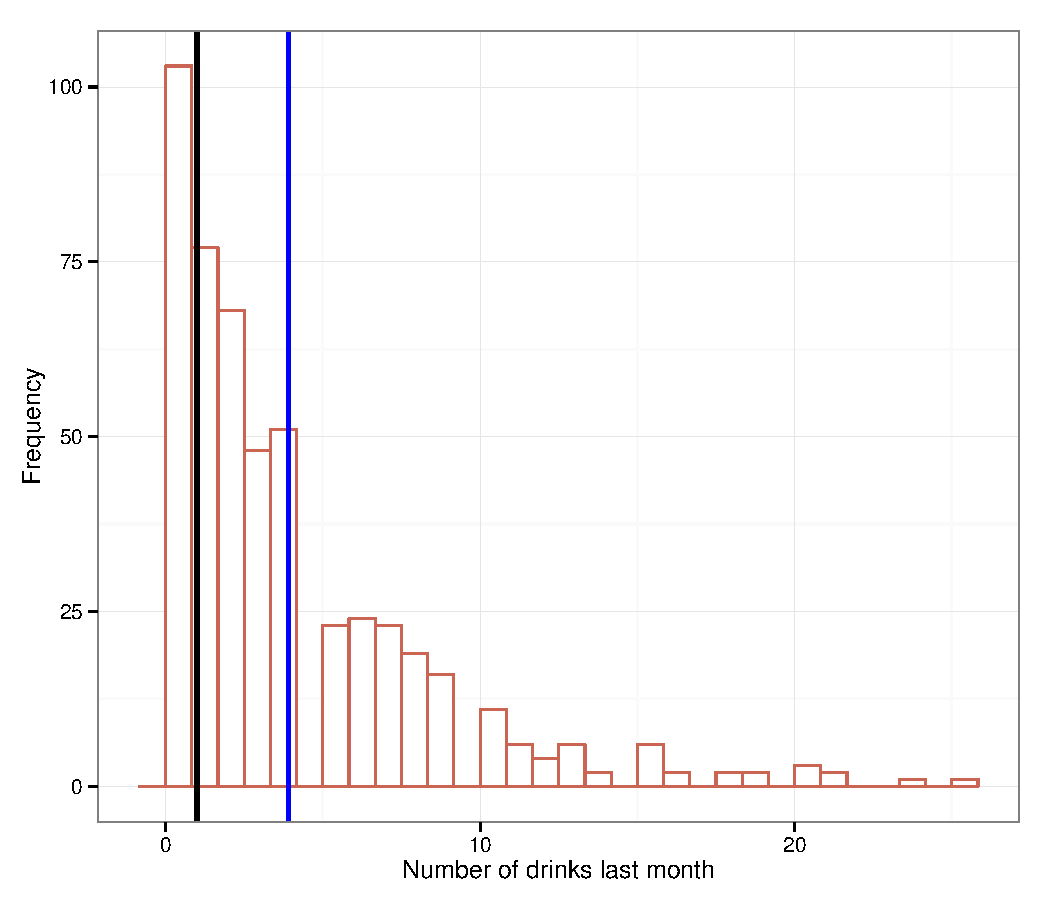
\includegraphics[width=\maxwidth]{figure/unnamed-chunk-6-1} 

}



\end{knitrout}
\end{frame}

\begin{frame}
\frametitle{Variability}
\begin{knitrout}
\definecolor{shadecolor}{rgb}{0.969, 0.969, 0.969}\color{fgcolor}

{\centering 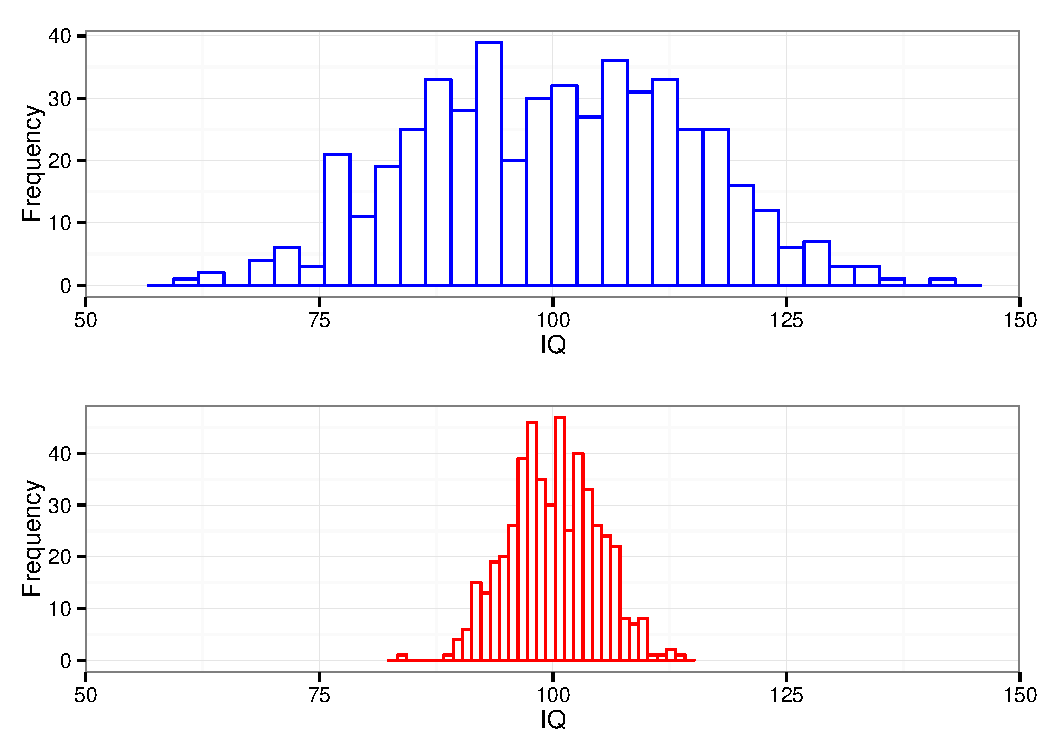
\includegraphics[width=\maxwidth]{figure/unnamed-chunk-7-1} 

}



\end{knitrout}
\end{frame}

\begin{frame}
\frametitle{Measures of variability}

Range

\vspace{.5cm}

Interquartile range ($Q_1$, $Q_2$, $Q_3$)

\vspace{.5cm}

Standard Deviation and Variance
$$
s = \sqrt{\frac{\sum{X_i - \bar{X}}}{n - 1}}
$$
$$
s^2 = \frac{\sum{X_i - \bar{X}}}{n - 1}
$$
\end{frame}

\begin{frame}
\begin{knitrout}
\definecolor{shadecolor}{rgb}{0.969, 0.969, 0.969}\color{fgcolor}

{\centering 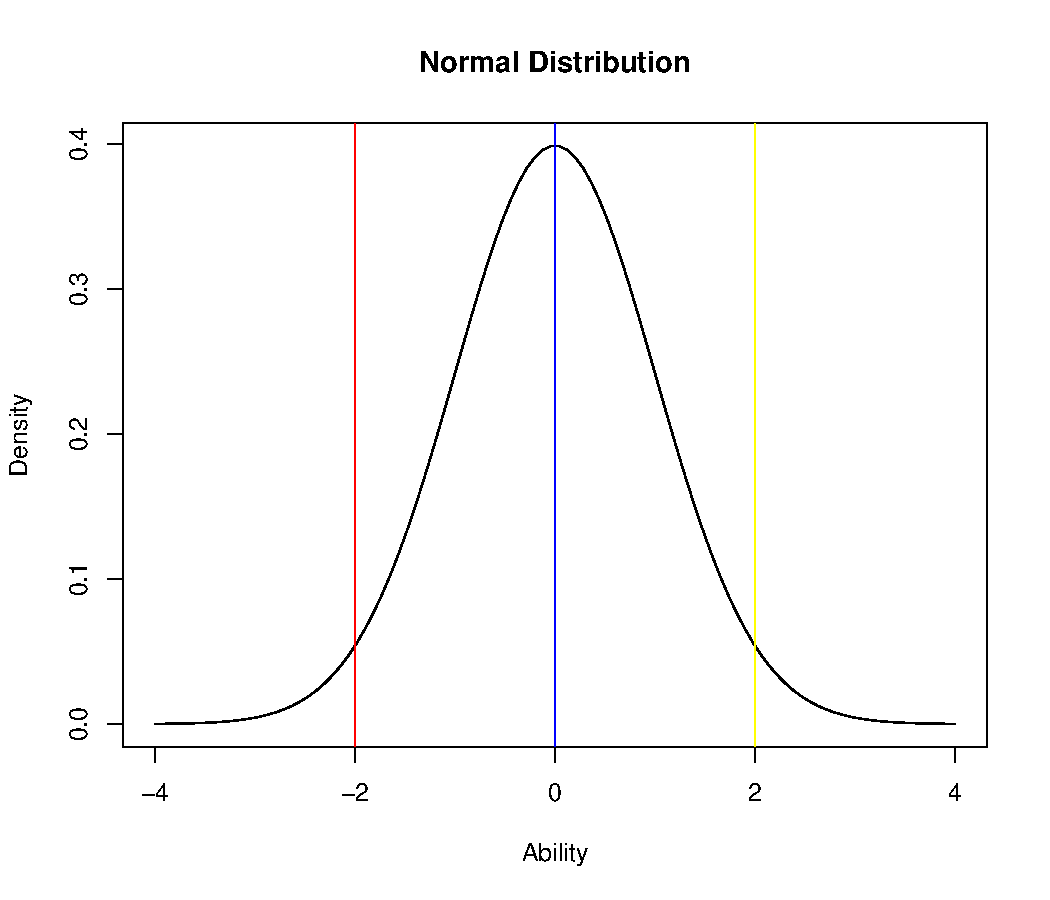
\includegraphics[width=\maxwidth]{figure/unnamed-chunk-8-1} 

}



\end{knitrout}
\end{frame}

\begin{frame}
\frametitle{Distributions, skewness, kurtosis}
  \begin{itemize}
    \item What is a probability distribution
  \begin{itemize}
    \item Assigns a probability, likeliness of occurence, of a score of all possible scores
    \item May be parametric or non-parametric
  \end{itemize}
  \item What skew might you expect these outcomes to look like?
    \begin{itemize}
    \item Reaction time in a psychological experiment
    \item Number of children in a family
    \item Scores on an easy test
    \item Height in Iceland
    \end{itemize}
  \item Platykurtic, mesokurtic, and leptokurtic
  \item Plot your data, rely less on statistics!
  \end{itemize}
\end{frame}

\begin{frame}
\frametitle{Shapes of distributions}
\begin{center}
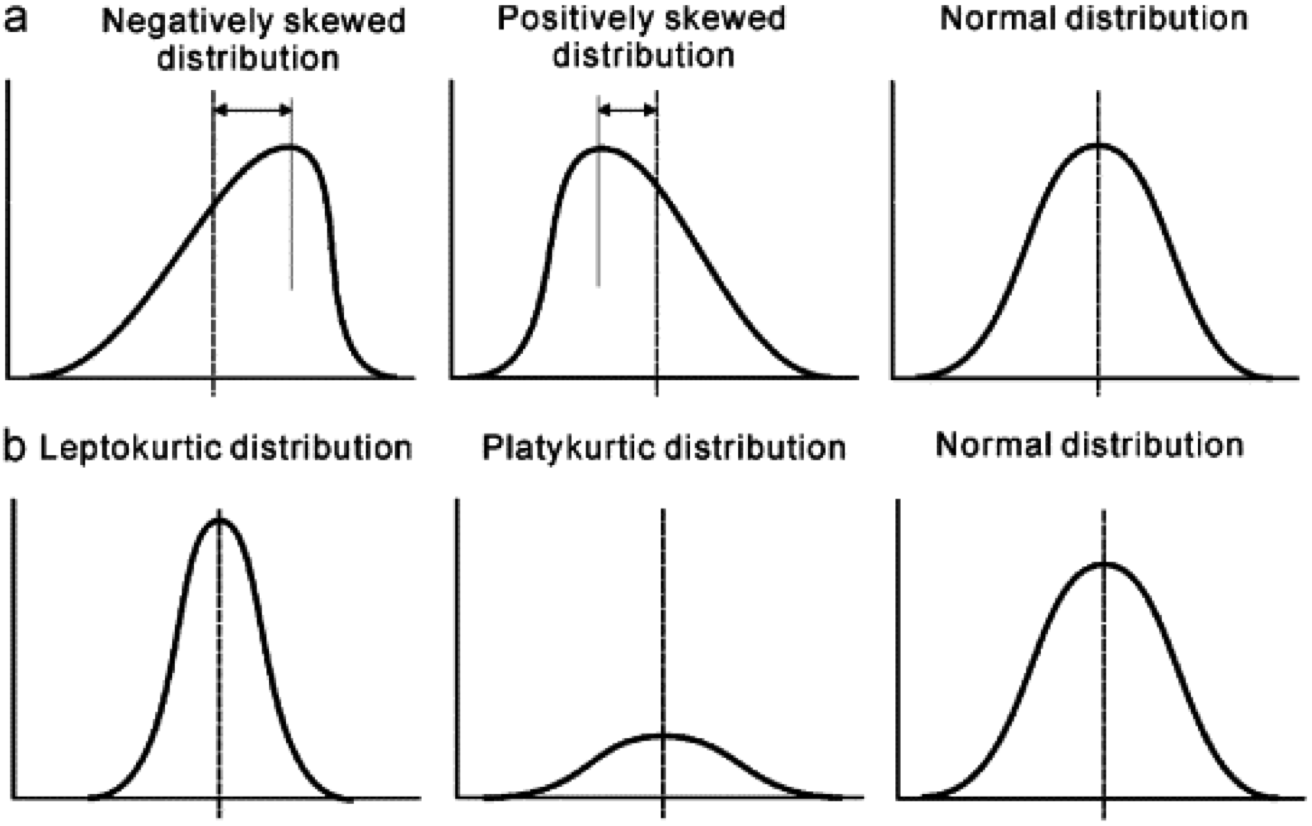
\includegraphics[scale = .5]{images/distributions.png}
\end{center}
\end{frame}

\begin{frame}
\frametitle{Normal Distribution}
\begin{knitrout}
\definecolor{shadecolor}{rgb}{0.969, 0.969, 0.969}\color{fgcolor}

{\centering 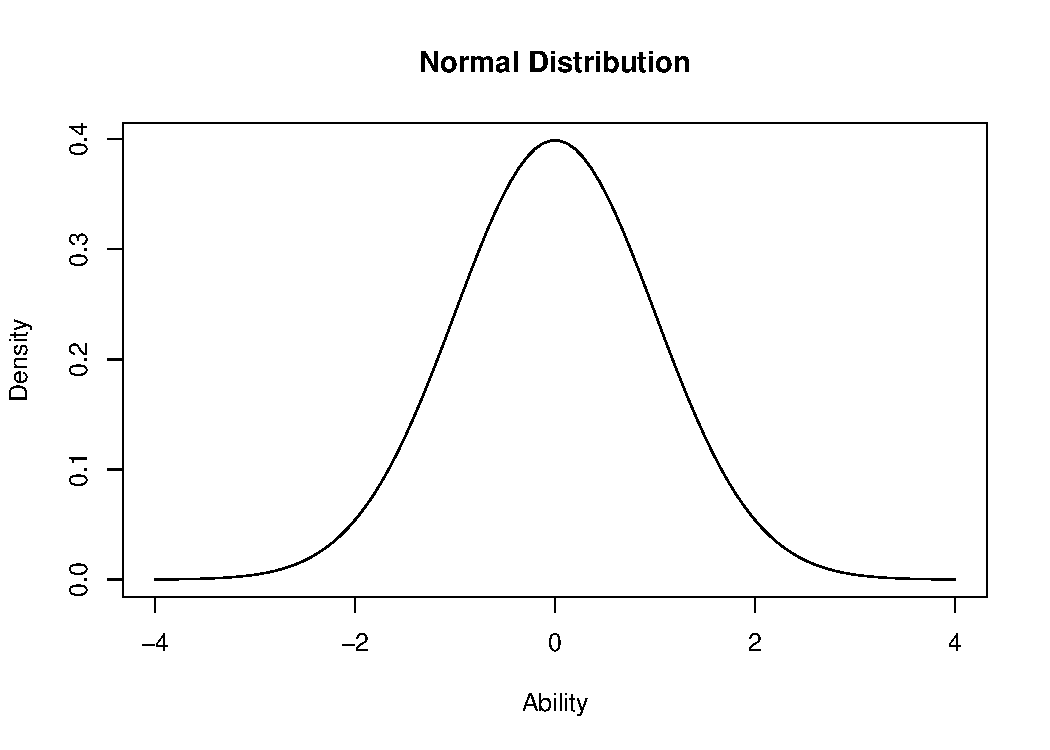
\includegraphics[width=\maxwidth]{figure/unnamed-chunk-9-1} 

}



\end{knitrout}
\end{frame}

\begin{frame}
\frametitle{IQ - 1 Standard Deviation}
\begin{knitrout}
\definecolor{shadecolor}{rgb}{0.969, 0.969, 0.969}\color{fgcolor}

{\centering 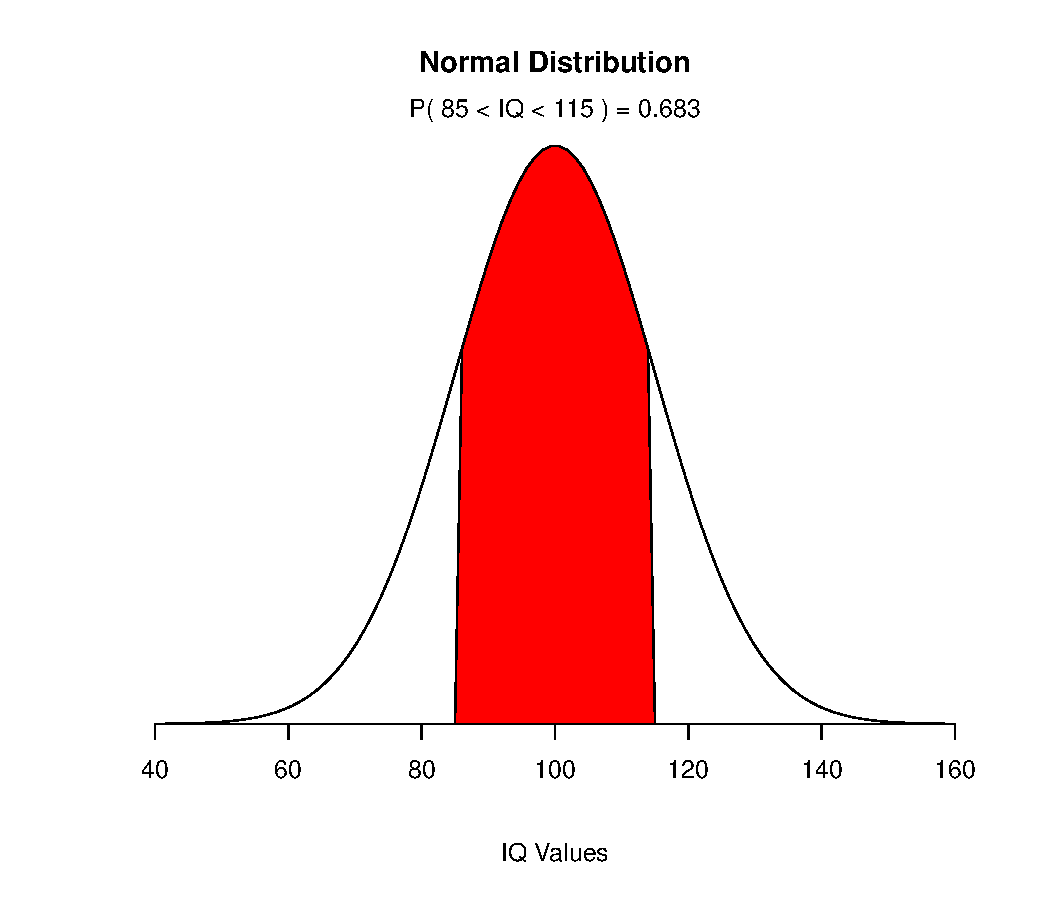
\includegraphics[width=\maxwidth]{figure/unnamed-chunk-10-1} 

}



\end{knitrout}
\end{frame}

\begin{frame}
\frametitle{IQ - 2 Standard Deviation}
\begin{knitrout}
\definecolor{shadecolor}{rgb}{0.969, 0.969, 0.969}\color{fgcolor}

{\centering 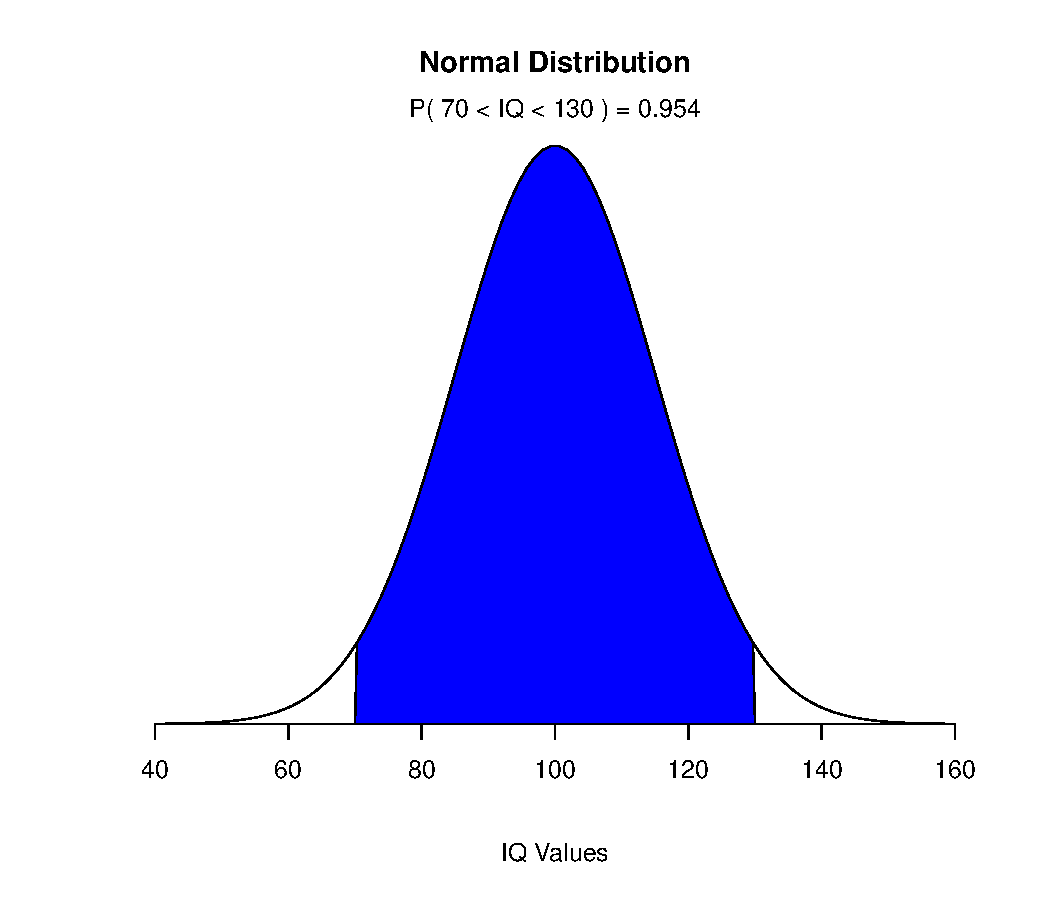
\includegraphics[width=\maxwidth]{figure/unnamed-chunk-11-1} 

}



\end{knitrout}
\end{frame}

\begin{frame}
\frametitle{IQ - 3 Standard Deviation}
\begin{knitrout}
\definecolor{shadecolor}{rgb}{0.969, 0.969, 0.969}\color{fgcolor}

{\centering 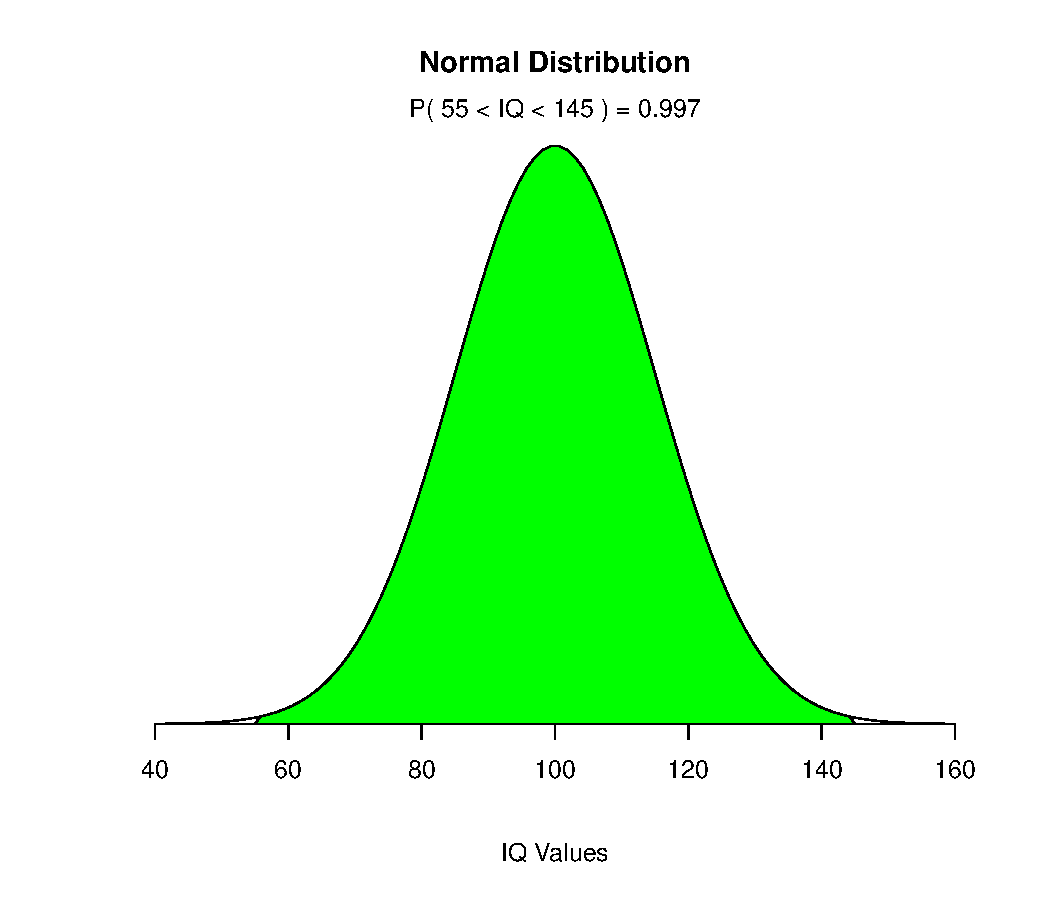
\includegraphics[width=\maxwidth]{figure/unnamed-chunk-12-1} 

}



\end{knitrout}
\end{frame}

\begin{frame}
\frametitle{Characteristics of the Normal distribution}
\begin{center}
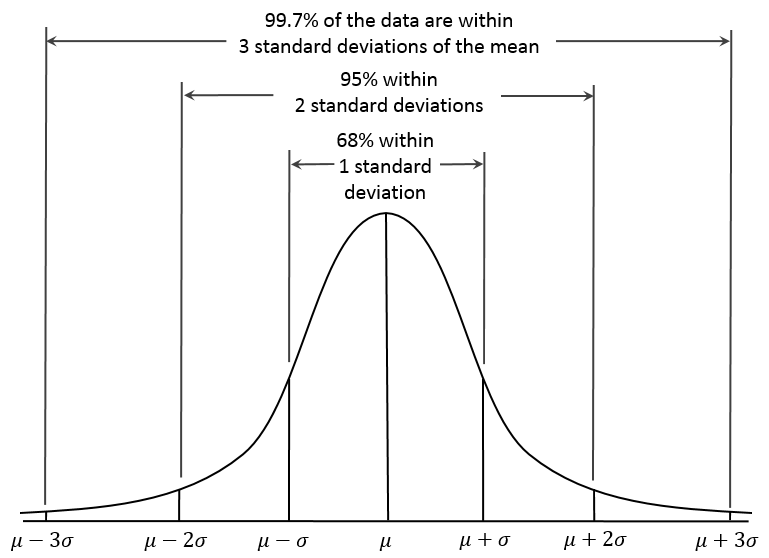
\includegraphics[scale = .5]{images/normal.png}
\end{center}
\end{frame}

\begin{frame}
\frametitle{Z-distribution}

\begin{itemize}
  \item<1-> The standard normal distribution is known as the z-distribution
  \item<2-> \textcolor{red}{What is the mean and the standard deviation of this distribution?}
  \item<3-> All normal distributions can be converted to the z-distribution
  \item<4-> A raw score can be converted to a z-score.
  \item[]<5-> \begin{center}$z = \frac{x - \mu}{\sigma}$\end{center}
\end{itemize}
\end{frame}

\begin{frame}
  \frametitle{SAT}
  
  The SAT is an aptitude test that high schools take. It is one of the criteria that is used in a college's decision to admit a student. It is composed of a math and a verbal section. Each has a mean of 500 and a standard devation of 110 and is normally distributed. 
  \begin{itemize}
  \item<1-> What are the scores on the test that corresponds to 3, 2, 1, 0, -1, -2, -3 standard deviations?
  \item<2-> Assume 1000 people took the SAT,
  \begin{itemize}
    \item<3-> If Jon got a 700 on the math section, how many people scored above him?
    \item<4-> If 300 people scored below Anna on the verbal section, what was Anna's score?
    \item<5-> How many people got scores between 390 and 610?
    \item<6-> If Sigga got a 350 on the math section, how many people scored below her?
    \item<7-> If Einar was in the 98\% percentile in math, what was Einar's score?
  \end{itemize}
  \end{itemize}
\end{frame}


\begin{frame}
\frametitle{Other standard scores}
\begin{itemize}
  \item<1-> \textcolor{red}{T scores} have a mean of 50 and a standard deviation of 10.
    \begin{itemize}
      \item<2-> What would T scores of 30 and 70 be as z-scores?
    \end{itemize}
    \item<3-> \textcolor{red}{stanine}, range from 1 to 9, are centered at 5 with a standard deviation of 2. Each stanine, corresponds to 1/2 a standard deviation and the 5th stanine is at the mean.
      \begin{itemize}
        \item<4-> If you were in the 3rd stanine, what would your z-score be?
        \item<5-> How many people would be below you?
        \item<6-> What percent of the people are between the 3rd and the 6th stanines?
      \end{itemize}
      \item<7-> Various linear and non-linear transformations are done to create scores and scores may be normalized.
\end{itemize}
\end{frame}

\begin{frame}
\frametitle{What is a correlation?}
\begin{itemize}
  \item Is it an association?
  \item Does it imply causation?
  \item Is a correlation necessary for causation?
  \item Does it need linearity?
  \item Is it affected by variability?
  \item Is it affected by outliers?
  \item Is it related to the simple linear regression?
\end{itemize}
\end{frame}

\begin{frame}
\frametitle{What is the correlation?}
\begin{knitrout}
\definecolor{shadecolor}{rgb}{0.969, 0.969, 0.969}\color{fgcolor}

{\centering 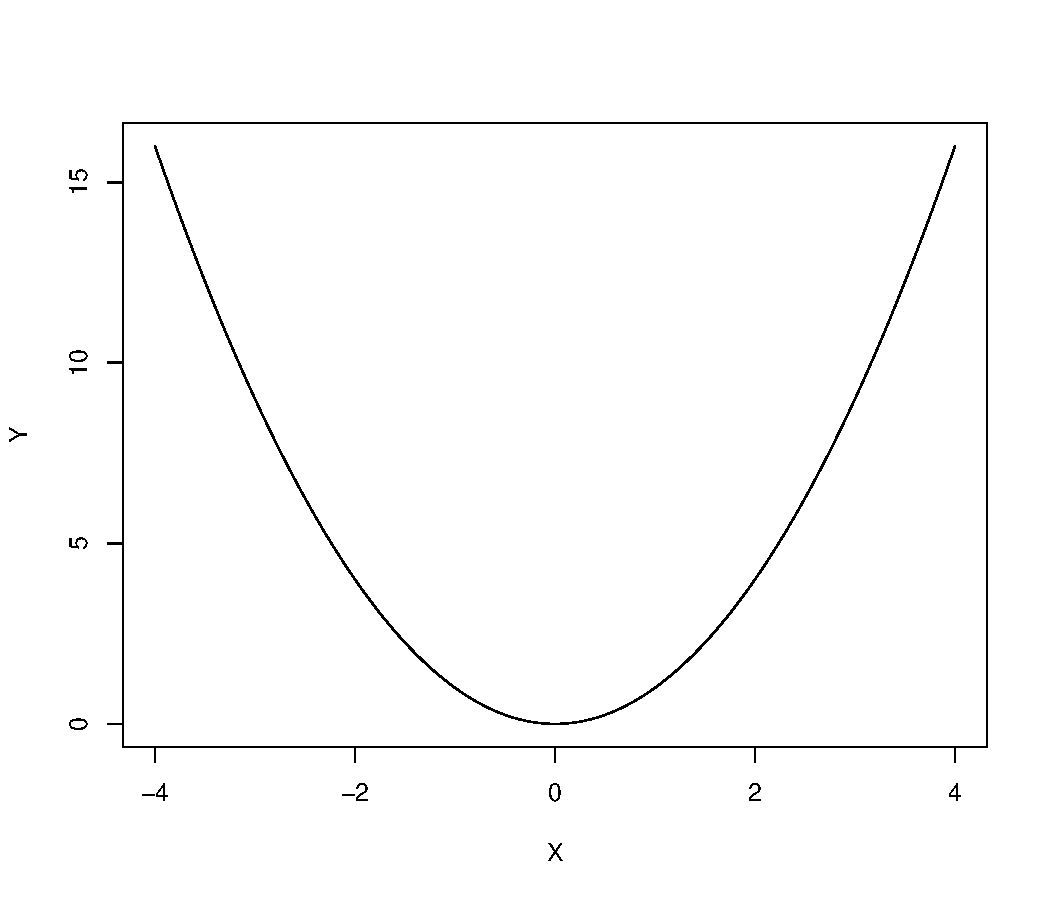
\includegraphics[width=\maxwidth]{figure/unnamed-chunk-13-1} 

}



\end{knitrout}
\end{frame}

\begin{frame}
\frametitle{Correlation}
$$
\frac{\sum(X - \bar{X})(Y - \bar{Y})}{\sqrt{\sum(X - \bar{X})^2\sum((Y - \bar{Y})^2}}
$$
\end{frame}

\begin{frame}
\frametitle{Calculating correlations}
\begin{tabular}{lll}
\hline
&X	& Y \\
\hline
&5 &	6 \\
&3	&0 \\
&1	&0 \\
\hline
Mean &	3	&2 \\
\hline
\end{tabular}
\end{frame}

\end{document}
